\documentclass{article}
\usepackage[UTF8]{ctex}
\usepackage{newtxtext}
\usepackage{geometry}
\usepackage[dvipsnames,svgnames]{xcolor}
\usepackage[strict]{changepage} % 提供一个 adjustwidth 环境
\usepackage{framed} % 实现方框效果
\usepackage{setspace}
\usepackage{tikz}
\usepackage{tcolorbox}
\usepackage{amsmath}
\usepackage{graphicx}
\usepackage{wrapfig}
\usepackage{float}
\usepackage{booktabs}
\usepackage{amssymb}
\geometry{a4paper,centering,scale=0.8,left=2.0cm,right=2.0cm,top=2.0cm,bottom=2.0cm}

\definecolor{blueshade}{rgb}{0.95,0.95,1} % 文%本框颜色
\definecolor{greenshade}{rgb}{0.90,0.99,0.91} % 绿色文本框,竖线颜色设为 Green
\definecolor{redshade}{rgb}{1.00,0.90,0.90}% 红色文本框,竖线颜色设为 LightCoral
\definecolor{brownshade}{rgb}{0.99,0.97,0.93} % 莫兰迪棕色,竖线颜色设为 BurlyWood
\definecolor{yellowshade}{rgb}{1,0.945,0.7255}%米黄色
\definecolor{DarkYellow}{rgb}{0.7843,0.61176,0.0549}

\newenvironment{formal}[2][greenshade]{%
\def\FrameCommand{%
\hspace{1pt}%
{\color{#2}\vrule width 2pt}%
{\color{#1}\vrule width 4pt}%
\colorbox{#1}%
}%
\MakeFramed{\advance\hsize-\width\FrameRestore}%
\noindent\hspace{-4.55pt}% disable indenting first paragraph
\begin{adjustwidth}{}{7pt}%
\vspace{2pt}\vspace{2pt}%
}
{
\vspace{2pt}\end{adjustwidth}\endMakeFramed%
}



\title{\Huge 证券投资学-第五次作业    \\\large made by  \LaTeX}
\author{刘宇晨\hspace*{25pt}20002515\\计金(双)200}


%\begin{tcolorbox}
%    [colback=Emerald!10,colframe=cyan!40!black,title=\textbf{公式}]
%\end{tcolorbox}

\begin{document} 
\begin{figure}[H]
    \begin{center}
        
\includegraphics[width=0.3\textwidth]{logo.jpeg}
        \maketitle
    \end{center}
\end{figure}
\thispagestyle{empty}
\clearpage
\pagenumbering{arabic}
\section*{\center 第二十四章作业}
\subsection*{习题9}
a.计算每只股票的下列指数:

\textbf{i.求$\alpha$}:通过回归模型中的公式可立即求出$\alpha$
\[r_p=\alpha+\beta \times (r_M-r_f)\]

所以$\alpha_A=1\%,\alpha_B=2\%$

\textbf{ii.求信息比率:}信息比率是用投资组合$\alpha$除以该组合的非系统性风险,也称为“循迹误差”
\[\text{信息比率}=\frac{\alpha_P}{\sigma (e_P)}\]

所以$\text{信息比率}_A=\frac{1\%}{10.3\%}=9.71\%,\text{信息比率}_B=\frac{2\%}{19.1\%}=10.47\%$

\textbf{iii.求夏普比率:}
\[\text{夏普比率}=\frac{\overline{r_P}-\overline{r_f} }{\sigma_P}\]

将题目所给的信息($r_f=6\%,r_M=14\%$)带入回归模型,分别计算$A,B$的超额收益,再带入公式得
:$\text{夏普比率}_A=\frac{10.6\%}{21.6\%}=49.07\%,\text{夏普比率}_B=\frac{8.4\%}{24.9\%}=33.73\%$

\textbf{iv.求特雷纳测度:}单位风险的超额收益
\[T^2=\frac{\overline{r_P}-\overline{r_f}}{\beta_P}\]

所以$T^2_A=\frac{10.6\%}{1.2}=8.33\%,T^2_B=\frac{8.4\%}{0.8}=10.5\%$

b.在下列情况下,哪只股票是最佳选择

\textbf{i.这是投资者唯一持有的风险资产:}
如果是唯一持有的风险资产,那么应该对比两只股票的夏普比率,因为夏普比率权衡的是风险溢价和风险,对于单个
投资资产,只用将这两个值得比例权衡好即可。由于只投资了一个股票,所以非系统性风险尚未被分散,
所以应选夏普比率大的股票,即选股票$A$。

\textbf{ii.这只股票将与投资者的其他债券资产组合混合,是目前市场指数基金的一个独立组成部分。}
可以用$M^2$测度来比较$A,B$两只股票。因为股票要和市场指数基金组合,所以用$M^2$测度的风险调整方法
很容易解释特定投资组合与市场基准指数之间的收益率差额。组合$P$的$M^2$测度如下:
\[M^2_P=r_{P^*}-r_M\]

构建资本配置线,并将市场平均回报率带入,由于题目没有给市场的标准差,如果无法求得$M^2$:
\nonumber
\begin{align}
    \begin{cases}
        10.6\%&=6\%+21.6\% \times k_1 \rightarrow\hspace*{25pt} k_1=0.21296\\
        8.4\%&=6\%+24.9\% \times k_2 \rightarrow \hspace*{25pt} k_2=0.09639\\
    \end{cases}
\end{align}

只能用特雷纳测度来评判,选股票$B$。

\textbf{iii.这是投资者目前正在分析以便构建一积极的管理型股票资产组合的众多股票中的一种。}
对于构建股票组合中的股票,不能只用夏普比率来评价股票,因为投资组合的非系统性风险被大大分散,系统性风险成为
风险的相关测度。所以应用单位风险的超额收益来分析,即特雷纳测度。所以应选股票$B$。

\subsection*{习题11}
a.对比经理的收益率和市场上的收益率,设经理的投资组合为$P$,市场的投资组合为$M$:
\begin{align}
    r&=\sum w_i \times r_i\\
    r_P&=0.7 \times 2\% + 0.2\times 1\%+0.1\times 0.5\%=1.65\%\\
    r_M&=0.6 \times 2.5\% + 0.3\times 1.2\%+0.1\times 0.5\%=1.91\%\\
    r_P-r_M&=1.65\%-1.91\%=-0.26\%
\end{align}

经理的收益率小于市场收益率0.26\%,所以为不良表现

b.计算债券选择在相对业绩表现中起的作用:先计算真实收益与市场收益的差值,然后分别乘以实际权重。
\[\text{债券选择的差值}=0.7 \times (2\%-2.5\%) + 0.2\times (1\%-1.2\%)=-0.39\%\]

c.先计算资产配置在相对业绩表现中的作用,用经理所选比例和基准比例的差值乘以市场收益。
再将资产配置的差值与债券选择的差值相加,即可得到不良表现。
\[\text{资产配置的差值}=2.5\% \times (0.7-0.6) + 1.2\%\times (0.2-0.3)=0.13\%\]

所以,相加之后有:
\begin{align}
    \text{超额业绩}&=\text{债券选择的差值}+\text{资产配置的差值}\\
    -0.26\%&=-0.39\%+0.13\%
\end{align}

所以选股与配置各自的贡献的总和等于她的相对于基准的超额收益。
\clearpage
\subsection*{习题12}
a.类似上一题,设经理的投资组合为$P$,市场的投资组合为$M$:
\begin{align}
    r_P&=0.3 \times 20\% + 0.1\times 15\%+0.4\times 10\%+0.2 \times 5\%=12.5\%\\
    r_M&=0.15 \times 12\% + 0.3\times 15\%+0.45\times 14\%+0.1 \times 12\%=13.8\%\\
    r_P-r_M&=12.5\%-13.8\%=-1.3\%
\end{align}

经理的收益率小于市场收益率1.3\%,所以为不良表现

b.类似上一题,计算国家配置决策的差值
\begin{align}
    \text{国家配置决策的差值}=&(12\%-13.8\%) \times (0.3-0.15) + =(15\%-13.8\%) \times (0.1-0.3) +\\
    &(14\%-13.8\%) \times (0.4-0.45) +(12\%-13.8\%) \times (0.2-0.1) =  -0.7\%
\end{align}


c.类似上一题,计算在其他国家股票选择方面的差值,在每一个国家,差值等于经理所选的比例乘以经理的收益率与市场的收益率的差值。
\[\text{股票选择方面的差值}=(20\%-12\%) \times 0.3 + =(15\%-15\%) \times 0.1 +
(10\%-14\%) \times 0.4 +(12\%-5\%) \times 0.2 = -0.6\% \]

所以,相加之后有:
\[ \text{超额业绩}=\text{国家配置决策的差值}+\text{股票选择方面的差值}=(-0.7\%)+(-0.6\%)=-1.3\%\]

所以国家配置与债券选择决策的价值总和等于总的超额收益的值。
\subsection*{CFA考题-11}
先计算时间加权平均收益:
\begin{align}
    \text{终值}&=\prod_{i=1}^{n}(1+r_i)\\
    g&=\text{终值}^{1/n}-1\\
    \therefore\text{终值}&=(1+15\%)\times (1+10\%)=1.265\\
    g&=(1.265)^{1/2}-1=0.1247\%
\end{align}

再计算美元加权收益率:用现金流贴现法,令现金流入的现值与现金流出的现值相等。
\[-50000-\frac{50000}{1+r}=\frac{(50000\times 1.265)+(50000\times 1.1)}{(1+r)^2}\]

解得$r=11.71\%$。
\clearpage
\section*{\center 第二十六章作业}
\subsection*{习题14}
a.如果要对冲下个月的市场敞口,需要多少份合约?购入还是售出?

当确信下个月的阿尔法是正的,针对错误定价建立一个纯赌局。由于阿尔法为正,\textbf{应该卖出合约}
\[\text{对冲比率}=\frac{2000000}{250 \times 1000}\times 0.75=6\text{份合约}\]

b.对冲基金月收益率的标准差应该等于股票的残差标准差,因为残差标准差是公司特定风险,是非系统性风险
无法被对冲消除。所以标准差应为6\%。

c.下个月市场中性策略亏损的概率有多大?

在进行市场中性策略时,对利率敞口进行套期保值。如果收益率价差返回到常态时,即下个月
$Waterwork$公司股票的阿尔法为基金经理预测的阿尔法时,即公司的收益率等于或大于普尔500指数加上阿尔法,持有市场中性头寸即可获利。此时
\[r=\alpha +r_f=2\%+0.5\%=2.5\%\]
标准差为6\%,所以
\begin{align}
    r&\sim N(2.5\%,6\% ^2)\\
    P\{r<0\}&=P\{\frac{r-2.5\%}{6\%}<-\frac{2.5\%}{6\%}\}\\
    &=N (-\frac{2.5\%}{6\%})=33.846112\%
\end{align}
\begin{figure}[H]
    \begin{center}
        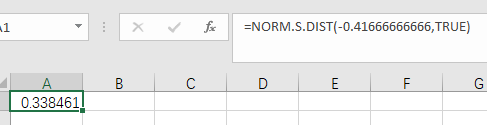
\includegraphics[width=1\textwidth]{1.png}
        \maketitle
    \end{center}
\end{figure}
\clearpage
\subsection*{习题17}
a. 缴纳激励费后联接基金投资人的收益率:

(由于收益率都大于零,所以可以把激励费比率的乘数从$\sum$中提取出来)
\[r_{FF}=(1-\text{激励费比率})^2\times \sum w_i r_i=12.8\%\]

b.假设持有$SA$基金的投资人,不用支付最初的激励费,那么收益率:
\[r_{SA}=(1-\text{激励费比率})\times \sum w_i r_i=16\%\]

所以年底他的组合价值为
\[V=300\times (1+16\%)=348\text{万美元}\]

c.证明收益率超出FF的部分是联接基金收取的激励费。
\begin{align}
    r_{FF}&=r\times (1-20\%) \times (1-20\%)\\
    r_{SA}&=r\times (1-20\%)\\
    \varDelta r&=r_{SA}-r_{FF}\\
    &=[r\times (1-20\%)](1-(1-20\%))\\
    &=20\% \times (r\times (1-20\%))=\text{联接基金收取的那一层激励费}
\end{align}


d.如果基金3的收益率为-30\%,由于最后收益率都$\leq 0$,所以都不抽取激励费:
\begin{align}
    r_{FF}&=\sum (1-\text{激励费比率}) w_i r_i \hspace*{25pt}(if\hspace*{15pt}  w_i r_i>0)=-2\%\\
    r_{SA}&= \sum w_i r_i=0\%
\end{align}

$FF$的投资人比$SA$的投资人情况更糟的原因是当每个对冲基金收益率大于$0$时,$FF$都会抽取$20\%$激励费,
导致总的收益率低于$SA$。

\end{document}

